\documentclass{article}
\usepackage[utf8]{inputenc}
\usepackage[german]{babel}
\usepackage{amsmath,amsthm,amssymb,mathrsfs}
\usepackage{geometry}
\usepackage[shortlabels]{enumitem}
\usepackage{wrapfig}
\usepackage{xcolor}

% For images
\usepackage{graphicx}
\usepackage{subcaption}
\graphicspath{ {./} }

% For tables not moving around
\usepackage{float}
\restylefloat{table}


\newcommand{\N}{\mathbb{N}}
\newcommand{\Q}{\mathbb{Q}}
\newcommand{\Z}{\mathbb{Z}}
\newcommand{\A}{\mathbb{A}}
\newcommand{\R}{\mathbb{R}}
\newcommand{\C}{\mathbb{C}}

\renewcommand{\i}{\text{i}}

\newcommand{\mat}[1]{\left(\begin{matrix}#1\end{matrix}\right)}
\newcommand{\smat}[1]{\left(\begin{smallmatrix}#1\end{smallmatrix}\right)}
\newcommand{\dmat}[1]{\begin{vmatrix}#1\end{vmatrix}}
\newcommand{\bmat}[2]{\left(\begin{array}{#1}#2\end{array}\right)}

\geometry{
	a4paper,
	total={170mm,240mm},
	left=20mm,
	top=30mm,
}

\definecolor{min1}{RGB}{49,77,133}
\definecolor{min2}{RGB}{0,141,137}
\definecolor{min3}{RGB}{0,201,105}
\definecolor{min4}{RGB}{207,185,61}
\definecolor{nomin}{RGB}{74,0,77}


\begin{document}
	\begin{table}[h]
		\centering
		\begin{tabular*}{\textwidth}{@{\extracolsep{\fill}}l c r }
			Moritz Seppelt & & Computational Physics\\ 
			194557 & \textbf{\Large{Hausaufgabe 3}} & vom 22.11.2021\\
			\hline 
		\end{tabular*}
	\end{table}
	\begin{figure}[H]
		\centering
		\subfloat[\centering Höhenkarte der Himmelblaufunktion (Werte leicht modifiziert: $f^{0.6}(\vec{x})$ dargestellt)]{{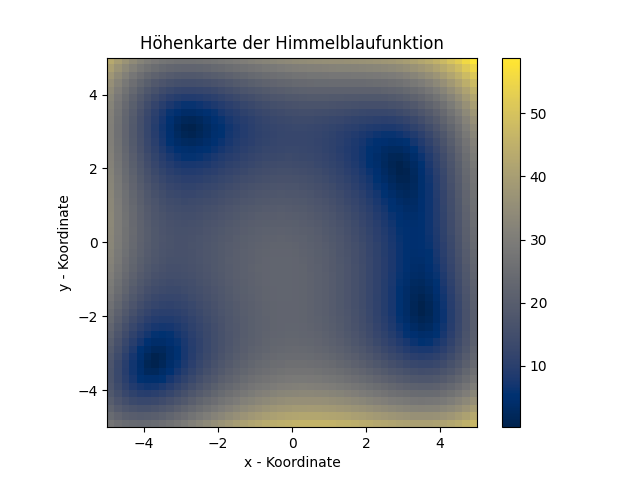
\includegraphics[scale=0.5]{fig3} }}
		\quad
		\subfloat[\centering Gefundenes Minimum in Abhängigkeit zum Startwert]{{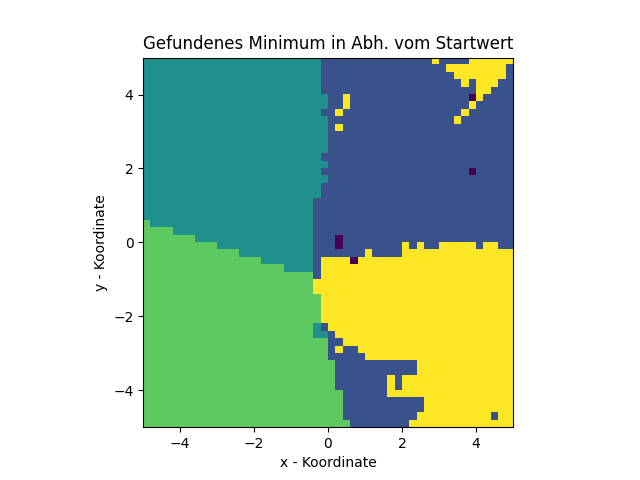
\includegraphics[scale=0.5]{fig1} }}
		\caption{Analyse Himmelblaufunktion im Überblick}
	\end{figure}
	Abbildung 1a stellt zum Überblick eine Höhenkarte der Himmelblaufunktion:
	$$f\smat{x\\y} = (x^2+y-11)^2+(x+y^2-7)^2$$
	dar. Dafür dass die Abbildung für kommende Argumente ansprechender ist, stelle ich statt $f(\vec{x}) \mapsto f^{0.6}(\vec{x})$ dar. Man sieht zum Beispiel recht gut die unten aufgeführten Minima $\vec{x}_{min_i}$.

	Auf Abbildung 1b erkennt man, für welchen Startort des Simplex, welches Minimum erreicht wird. Dabei ist das erreichte Minimum mit einer Farbe kodiert. Die Zuordnungen sind folgendermaßen:
	\begin{itemize}
		\item\textcolor{min1}{\textbf{Blauviolett}}: $\vec{x}_{min_1} = (3, 2)$
		\item\textcolor{min2}{\textbf{Türkis}}: $\vec{x}_{min_2} \approx (-2.805, 3.131)$
		\item\textcolor{min3}{\textbf{Grün}}: $\vec{x}_{min_3} \approx (-3.77, -3.283)$
		\item\textcolor{min4}{\textbf{Gelb}}: $\vec{x}_{min_4} \approx (3.584, -1.848)$
		\item\textcolor{nomin}{\textbf{Violett}}: Kein Minimum gefunden.
	\end{itemize} 
	
	Dabei sind große Teile der Färbungen sehr logisch. Zum Beispiel sind alle Pixel um $x_{min_3}$ auch \textcolor{min3}{\textbf{Grün}}. Dies spiegelt den intuitiven Fakt wieder, dass die Minima gefunden werden, die auch nah am Anfangsort liegen.
	
	Wir sehen jedoch auch 2 Ungewöhnlichkeiten. 1. \textcolor{min1}{\textbf{Blauviolett}} und \textcolor{min4}{\textbf{Gelb}} treten sehr gemischt auf. Anhand Abbildung 1a kann man erkennen, dass beide beide Minima in einem gemeinsamen Tal liegen, deren Hänge sehr steil sind. Damit kann es zum Beispiel bei dem \textcolor{min4}{\textbf{gelben}} Bereich bei ca. $(4, 4)$ die Simplexe über das nähere Minimum springen und dann sich in dem anderen Minimum im selben Tal wiederfinden. Eine ähnliche Erklärung kann man für den \textcolor{min1}{\textbf{blauvioletten}} Bereich bei ca $(1, -4)$ finden.
	
	2. Wir sehen leider auch 5 \textcolor{nomin}{\textbf{violette}} Punkte, die keinen der 4 Minima finden. Hier sind diese aufgelistet:
	\begin{center}
		\begin{tabular}{ c | c | c }
			$\vec{x}_{start}$ & $\vec{x}_{ende}$ & Iterationsschritte $N$ \\
			\hline
			$(3.980, 3.980)$ & $(3.204, 2.003)$ & 117\\
			$(3.980, 1.939)$ & $(2.958, 2.114)$ & 117\\
			$(0.306, 0.102)$ & $(3.293, 0.763)$ & 113\\
			$(0.306, -0.102)$ & $(3.331, 0.500)$ & 116\\
			$(0.714, -0.510)$ & $(3.388, 0.026)$ & 121
		\end{tabular}
	\end{center}

	Überraschenderweise läuft keiner dieser Anfangswerte in $N_{max} = 250$. Deshalb muss für jeden einzeln erklärt werden, warum der Simplex sich ``bewusst" dazu entscheidet dort ein Minimum zu platzieren. Man sieht schnell dass die $\vec{x}_{ende}$ von Zeilen 1 und 2 sehr nah an $\vec{x}_{min_1}$ liegen, nur nicht meine Abstandsbedingung von $$||\vec{x}_{min_i}-\vec{x}_{ende}||^2 < 0.1$$ erfüllen. Alle Anderen $\vec{x}_{ende}$ liegen auch in dem Tal von $\vec{x}_{min_1}$ und $\vec{x}_{min_4}$, welches (was man an er Höhenkarte erahnen kann) auch sehr flache Stück hat, die als Extreme missverstanden werden können. Außerdem fangen die Zeilen 3 bis 5 auch auf dem Plateau bei $(0, 0)$ an, wodurch die Simplexe auch anfangs schon künstlich verkleinert werden. Damit sind sie von Anfang an näher an der Abbruchbedingung.
	
	\begin{wrapfigure}[20]{r}{0.5\textwidth}
		\centering
		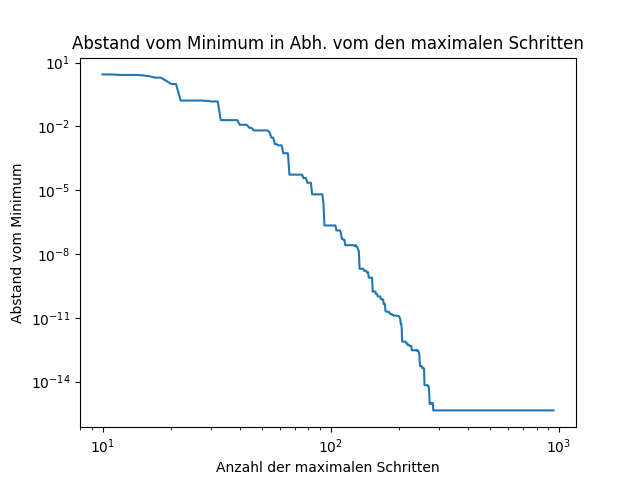
\includegraphics[width=0.5\textwidth]{fig2}
		\caption{Abstand vom Minimum in Abhängigkeit von den Schritten}
	\end{wrapfigure}

	Nun betrachten wir in Abbildung 2 für $\vec{x}_{start} = (-1, -1)$, in welchem Abstand sich der Simplex nach $N$ Schritten vom Minimum $\vec{x}_{min_3}$ befindet. Logischerweise kommt der Simplex näher heran, je länger er laufen darf. Außerdem wird der Abstand nach ca $N=300$ nicht mehr besser, ab diesen Zeit kontrahiert sich der Simplex nur noch und die leichte Abweichung lässt sich mit dem beschränkten Speicherplatz der Zahlen erklären. (Fehler auch in Größenordnung $10^{-14}$). Je nachdem ob nur gespiegelt oder gleich expandiert wurde, sind die Verbesserungen pro Schritt natürlich unterschiedlich. Damit erklärt sich dann auch der Stark unterschiedliche Abfall. Außerdem sehen wir an der harten Ecke bei $N\approx300$ im Plot, dass das Minimum sehr schnell gefunden wurde, und der Simplex im Tal nicht lange herumsucht.

\end{document}
